\documentclass[a4paper,11pt]{article}
\usepackage[a4paper, margin=8em]{geometry}

% usa i pacchetti per la scrittura in italiano
\usepackage[french,italian]{babel}
\usepackage[T1]{fontenc}
\usepackage[utf8]{inputenc}
\frenchspacing 

% usa i pacchetti per la formattazione matematica
\usepackage{amsmath, amssymb, amsthm, amsfonts}

% usa altri pacchetti
\usepackage{gensymb}
\usepackage{hyperref}
\usepackage{standalone}

\usepackage{colortbl}

\usepackage{xstring}
\usepackage{karnaugh-map}

% imposta il titolo
\title{Appunti Sistemi Operativi}
\author{Luca Seggiani}
\date{2025}

% imposta lo stile
% usa helvetica
\usepackage[scaled]{helvet}
% usa palatino
\usepackage{palatino}
% usa un font monospazio guardabile
\usepackage{lmodern}

\renewcommand{\rmdefault}{ppl}
\renewcommand{\sfdefault}{phv}
\renewcommand{\ttdefault}{lmtt}

% circuiti
\usepackage{circuitikz}
\usetikzlibrary{babel}

% testo cerchiato
\newcommand*\circled[1]{\tikz[baseline=(char.base)]{
            \node[shape=circle,draw,inner sep=2pt] (char) {#1};}}

% disponi il titolo
\makeatletter
\renewcommand{\maketitle} {
	\begin{center} 
		\begin{minipage}[t]{.8\textwidth}
			\textsf{\huge\bfseries \@title} 
		\end{minipage}%
		\begin{minipage}[t]{.2\textwidth}
			\raggedleft \vspace{-1.65em}
			\textsf{\small \@author} \vfill
			\textsf{\small \@date}
		\end{minipage}
		\par
	\end{center}

	\thispagestyle{empty}
	\pagestyle{fancy}
}
\makeatother

% disponi teoremi
\usepackage{tcolorbox}
\newtcolorbox[auto counter, number within=section]{theorem}[2][]{%
	colback=blue!10, 
	colframe=blue!40!black, 
	sharp corners=northwest,
	fonttitle=\sffamily\bfseries, 
	title=Teorema~\thetcbcounter: #2, 
	#1
}

% disponi definizioni
\newtcolorbox[auto counter, number within=section]{definition}[2][]{%
	colback=red!10,
	colframe=red!40!black,
	sharp corners=northwest,
	fonttitle=\sffamily\bfseries,
	title=Definizione~\thetcbcounter: #2,
	#1
}

% disponi codice
\usepackage{listings}
\usepackage[table]{xcolor}

\definecolor{codegreen}{rgb}{0,0.6,0}
\definecolor{codegray}{rgb}{0.5,0.5,0.5}
\definecolor{codepurple}{rgb}{0.58,0,0.82}
\definecolor{backcolour}{rgb}{0.95,0.95,0.92}

\lstdefinestyle{codestyle}{
		backgroundcolor=\color{black!5}, 
		commentstyle=\color{codegreen},
		keywordstyle=\bfseries\color{magenta},
		numberstyle=\sffamily\tiny\color{black!60},
		stringstyle=\color{green!50!black},
		basicstyle=\ttfamily\footnotesize,
		breakatwhitespace=false,         
		breaklines=true,                 
		captionpos=b,                    
		keepspaces=true,                 
		numbers=left,                    
		numbersep=5pt,                  
		showspaces=false,                
		showstringspaces=false,
		showtabs=false,                  
		tabsize=2
}

\lstdefinestyle{shellstyle}{
		backgroundcolor=\color{black!5}, 
		basicstyle=\ttfamily\footnotesize\color{black}, 
		commentstyle=\color{black}, 
		keywordstyle=\color{black},
		numberstyle=\color{black!5},
		stringstyle=\color{black}, 
		showspaces=false,
		showstringspaces=false, 
		showtabs=false, 
		tabsize=2, 
		numbers=none, 
		breaklines=true
}


\lstdefinelanguage{assembler}{ 
  keywords={AAA, AAD, AAM, AAS, ADC, ADCB, ADCW, ADCL, ADD, ADDB, ADDW, ADDL, AND, ANDB, ANDW, ANDL,
        ARPL, BOUND, BSF, BSFL, BSFW, BSR, BSRL, BSRW, BSWAP, BT, BTC, BTCB, BTCW, BTCL, BTR, 
        BTRB, BTRW, BTRL, BTS, BTSB, BTSW, BTSL, CALL, CBW, CDQ, CLC, CLD, CLI, CLTS, CMC, CMP,
        CMPB, CMPW, CMPL, CMPS, CMPSB, CMPSD, CMPSW, CMPXCHG, CMPXCHGB, CMPXCHGW, CMPXCHGL,
        CMPXCHG8B, CPUID, CWDE, DAA, DAS, DEC, DECB, DECW, DECL, DIV, DIVB, DIVW, DIVL, ENTER,
        HLT, IDIV, IDIVB, IDIVW, IDIVL, IMUL, IMULB, IMULW, IMULL, IN, INB, INW, INL, INC, INCB,
        INCW, INCL, INS, INSB, INSD, INSW, INT, INT3, INTO, INVD, INVLPG, IRET, IRETD, JA, JAE,
        JB, JBE, JC, JCXZ, JE, JECXZ, JG, JGE, JL, JLE, JMP, JNA, JNAE, JNB, JNBE, JNC, JNE, JNG,
        JNGE, JNL, JNLE, JNO, JNP, JNS, JNZ, JO, JP, JPE, JPO, JS, JZ, LAHF, LAR, LCALL, LDS,
        LEA, LEAVE, LES, LFS, LGDT, LGS, LIDT, LMSW, LOCK, LODSB, LODSD, LODSW, LOOP, LOOPE,
        LOOPNE, LSL, LSS, LTR, MOV, MOVB, MOVW, MOVL, MOVSB, MOVSD, MOVSW, MOVSX, MOVSXB,
        MOVSXW, MOVSXL, MOVZX, MOVZXB, MOVZXW, MOVZXL, MUL, MULB, MULW, MULL, NEG, NEGB, NEGW,
        NEGL, NOP, NOT, NOTB, NOTW, NOTL, OR, ORB, ORW, ORL, OUT, OUTB, OUTW, OUTL, OUTSB, OUTSD,
        OUTSW, POP, POPL, POPW, POPB, POPA, POPAD, POPF, POPFD, PUSH, PUSHL, PUSHW, PUSHB, PUSHA, 
				PUSHAD, PUSHF, PUSHFD, RCL, RCLB, RCLW, MOVSL, MOVSB, MOVSW, STOSL, STOSB, STOSW, LODSB, LODSW,
				LODSL, INSB, INSW, INSL, OUTSB, OUTSL, OUTSW
        RCLL, RCR, RCRB, RCRW, RCRL, RDMSR, RDPMC, RDTSC, REP, REPE, REPNE, RET, ROL, ROLB, ROLW,
        ROLL, ROR, RORB, RORW, RORL, SAHF, SAL, SALB, SALW, SALL, SAR, SARB, SARW, SARL, SBB,
        SBBB, SBBW, SBBL, SCASB, SCASD, SCASW, SETA, SETAE, SETB, SETBE, SETC, SETE, SETG, SETGE,
        SETL, SETLE, SETNA, SETNAE, SETNB, SETNBE, SETNC, SETNE, SETNG, SETNGE, SETNL, SETNLE,
        SETNO, SETNP, SETNS, SETNZ, SETO, SETP, SETPE, SETPO, SETS, SETZ, SGDT, SHL, SHLB, SHLW,
        SHLL, SHLD, SHR, SHRB, SHRW, SHRL, SHRD, SIDT, SLDT, SMSW, STC, STD, STI, STOSB, STOSD,
        STOSW, STR, SUB, SUBB, SUBW, SUBL, TEST, TESTB, TESTW, TESTL, VERR, VERW, WAIT, WBINVD,
        XADD, XADDB, XADDW, XADDL, XCHG, XCHGB, XCHGW, XCHGL, XLAT, XLATB, XOR, XORB, XORW, XORL},
  keywordstyle=\color{blue}\bfseries,
  ndkeywordstyle=\color{darkgray}\bfseries,
  identifierstyle=\color{black},
  sensitive=false,
  comment=[l]{\#},
  morecomment=[s]{/*}{*/},
  commentstyle=\color{purple}\ttfamily,
  stringstyle=\color{red}\ttfamily,
  morestring=[b]',
  morestring=[b]"
}

\lstset{language=assembler, style=codestyle}

% disponi sezioni
\usepackage{titlesec}

\titleformat{\section}
	{\sffamily\Large\bfseries} 
	{\thesection}{1em}{} 
\titleformat{\subsection}
	{\sffamily\large\bfseries}   
	{\thesubsection}{1em}{} 
\titleformat{\subsubsection}
	{\sffamily\normalsize\bfseries} 
	{\thesubsubsection}{1em}{}

% tikz
\usepackage{tikz}

% float
\usepackage{float}

% grafici
\usepackage{pgfplots}
\pgfplotsset{width=10cm,compat=1.9}

% disponi alberi
\usepackage{forest}

\forestset{
	rectstyle/.style={
		for tree={rectangle,draw,font=\large\sffamily}
	},
	roundstyle/.style={
		for tree={circle,draw,font=\large}
	}
}

% disponi algoritmi
\usepackage{algorithm}
\usepackage{algorithmic}
\makeatletter
\renewcommand{\ALG@name}{Algoritmo}
\makeatother

% disponi numeri di pagina
\usepackage{fancyhdr}
\fancyhf{} 
\fancyfoot[L]{\sffamily{\thepage}}

\makeatletter
\fancyhead[L]{\raisebox{1ex}[0pt][0pt]{\sffamily{\@title \ \@date}}} 
\fancyhead[R]{\raisebox{1ex}[0pt][0pt]{\sffamily{\@author}}}
\makeatother

\begin{document}
% sezione (data)
\section{Lezione del 15-10-25}

% stili pagina
\thispagestyle{empty}
\pagestyle{fancy}

% testo
Continuiamo la discussione dell'algoritmo \textbf{RM} (\textit{Rate Monotonic}).

Volevamo vedere gli effetti che si ottenevano quando si aumentava la pressione sulla CPU sfruttando questo algoritmo.
Prendiamo allora gli stessi processi $p_a$ e $p_b$ della scorsa lezione, ma raddoppiamo il tempo di esecuzione del processo $p_b$:
\begin{table}[H]
	\center \rowcolors{2}{white}{black!10}
	\begin{tabular} { c || c | c }
		\bfseries Processo & \bfseries $\Delta \mathbf{t}$ periodo & \bfseries $\mathbf{C}$ esecuzione \\
		\hline
		$p_a$ & 2 & 1 \\ 
		$p_b$ & 5 & 2
	\end{tabular}
\end{table}

\newpage

Simulando l'esecuzione si ha, colorando le linee di periodo come nello scorso esepmio: 
\begin{center}
	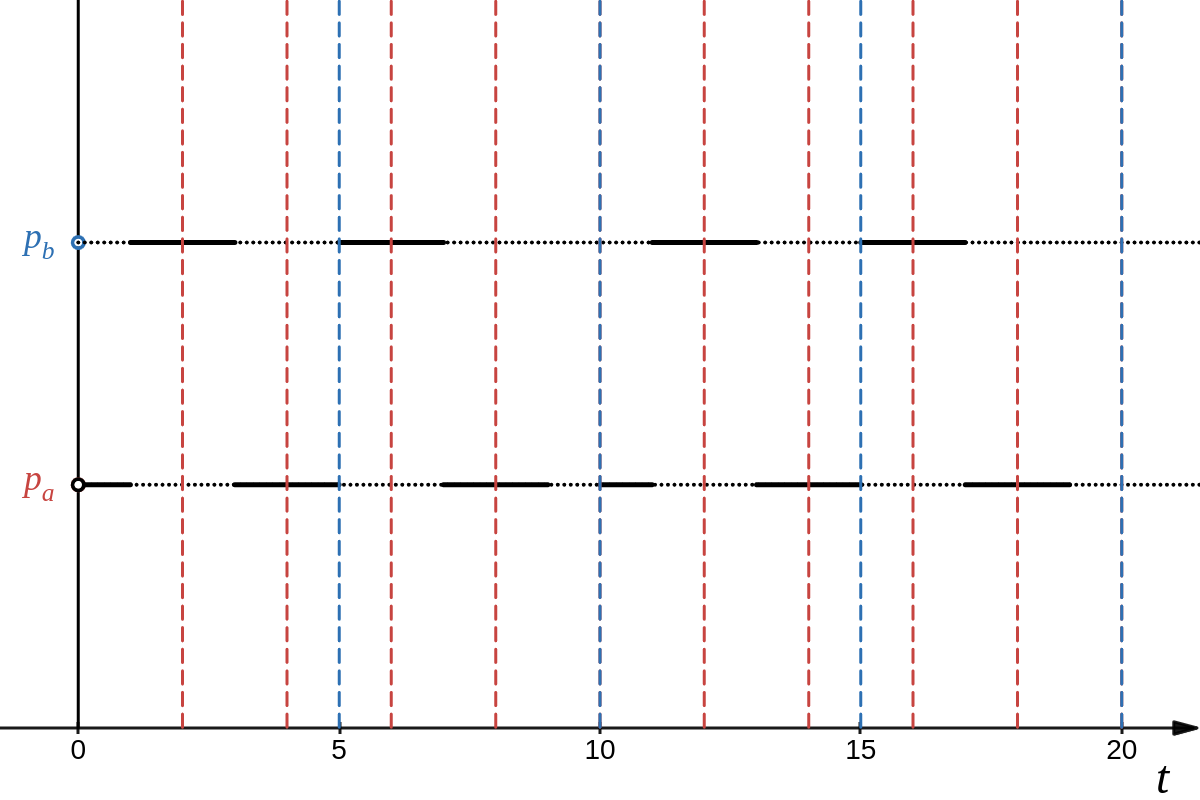
\includegraphics[scale=0.3]{../figures/rm_tight.png}
\end{center}

Vediamo quindi come siamo arrivati al 90\% di utilizzo della CPU, e come  il fatto che l'algoritmo è non preemptive significa che quando $p_b$ accede alla CPU, la tiene anche oltre la linea di periodo di $p_a$ (che ha comunque tempo di eseguire prima della linea successiva).

\subsubsection{Algoritmo RM "preemptive"}
Potremmo introdurre la preemption nell'algoritmo RM.
In questo caso, ad ogni periodo riportiamo in esecuzione il processo con priorità più alta.

\par\smallskip

Vediamo quindi la timeline che otteniamo applicando questa versione con preemption all'esempio della scorsa sezione: 
\begin{center}
	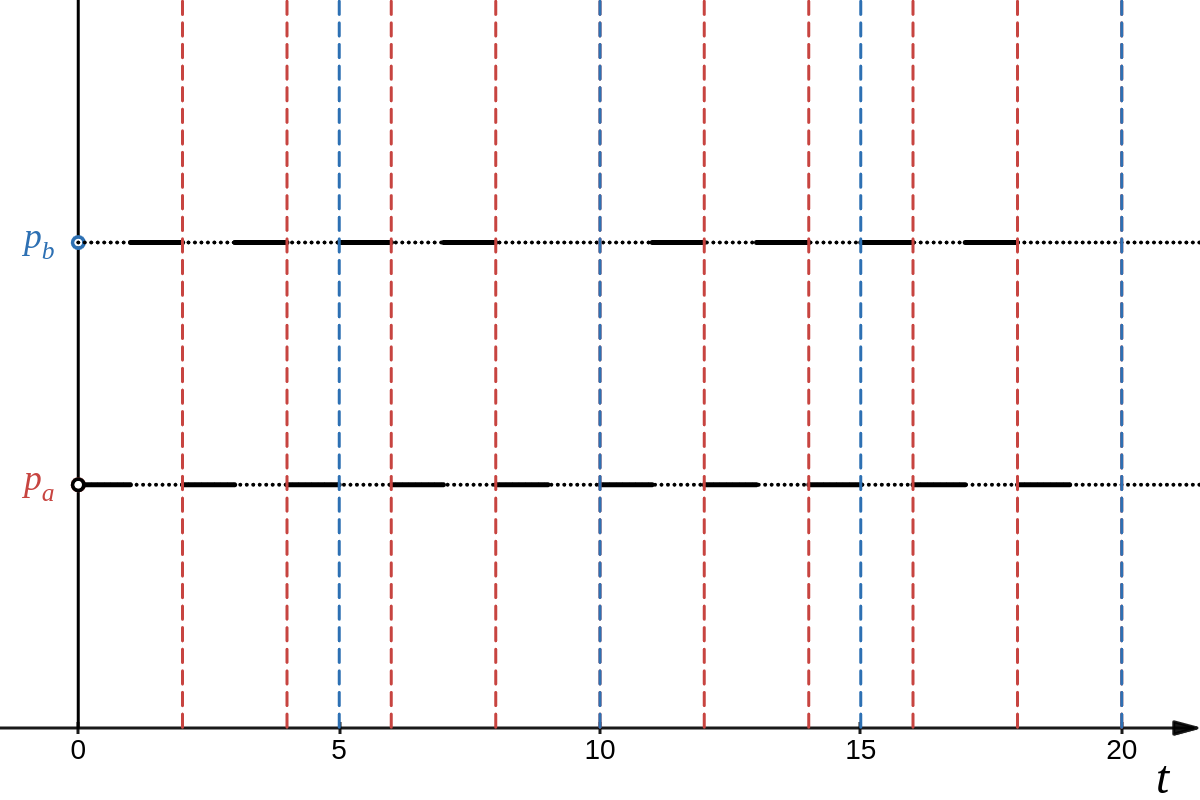
\includegraphics[scale=0.3]{../figures/rm_pre.png}
\end{center}

\par\smallskip

Notiamo che questo algoritmo di scheduling introduce un overhead maggiore della versione non preemptive, dato dai maggiori cambi di contesto. Inoltre, almeno in questo caso, non varia particolarmente in utilizzo CPU o in efficacia generale.

Comunque, possiamo osservare che mantiene i processi ancora più lontani dalla deadline, che è generalmente un comportamento desiderabile. 

\par\smallskip

Abbiamo quindi che per gli algoritmi a priorità \textit{static}, il RM è ottimo: se un insieme di processi è schedulabile a priorità statica in real-time, allora lo è con RM.
Di contro, se non è schedulabile con RM, non esiste nessun algoritmo a priorità statica che può schedularlo.

\subsection{Processi non schedulabili staticamente}
Approfondiamo cosa significa, per un insieme di processi, essere \textit{schedulabili a priorita statica}.
Prendiamo la tabella di processi: 
\begin{table}[H]
	\center \rowcolors{2}{white}{black!10}
	\begin{tabular} { c || c | c }
		\bfseries Processo & \bfseries $\Delta \mathbf{t}$ periodo & \bfseries $\mathbf{C}$ esecuzione \\
		\hline
		$p_a$ & 4 & 2 \\ 
		$p_b$ & 10 & 5
	\end{tabular}
\end{table}

Vediamo come ogni processo chiede di eseguire per metà del suo periodo.

Se usiamo la schedulazione RM in questo caso, otteniamo:
\begin{center}
	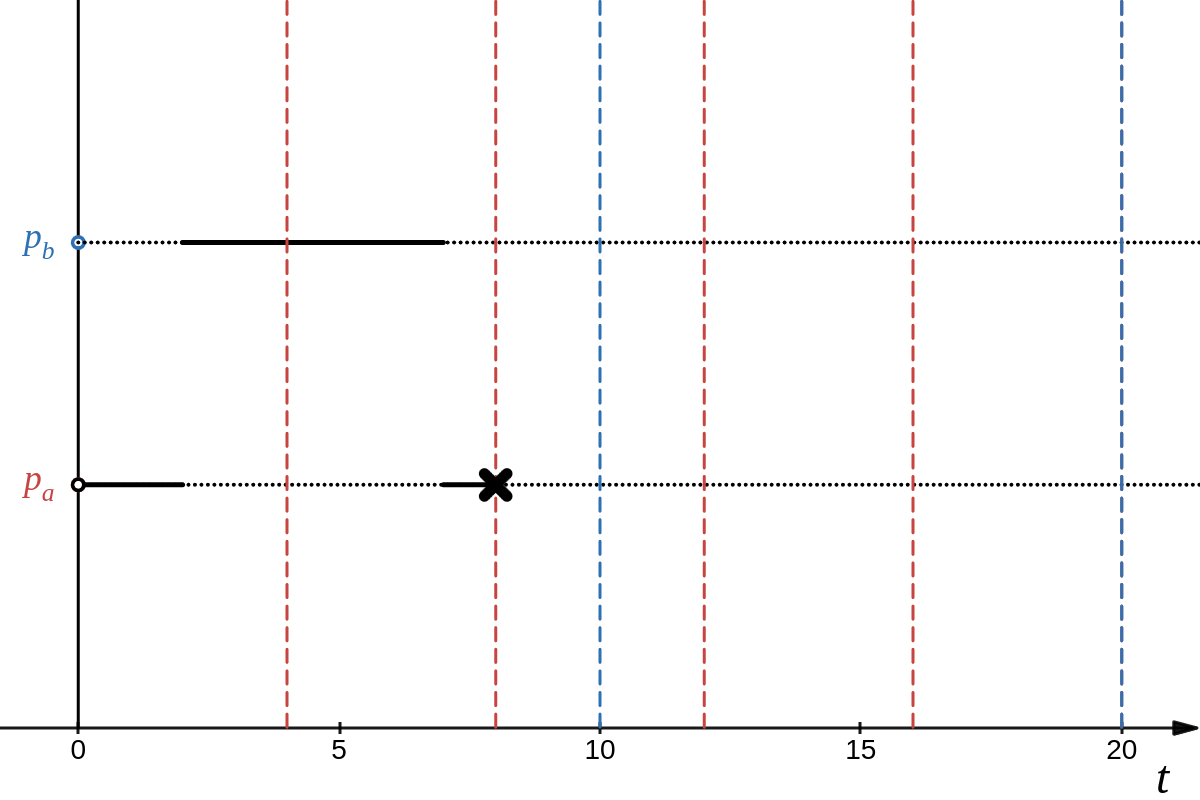
\includegraphics[scale=0.3]{../figures/rm_fail.png}
\end{center}

Dove all'istante $t = 8$ non siamo riusciti a completare il CPU burst di $p_a$, e si è quindi giunti ad un \textit{overflow}: un fallimento della schedulazione che non ha rispettato la deadline.

\newpage

Pensiamo allora di utilizzare l'algoritmo RM "preemptive" visto nella scorsa szione. In questo caso, si avrà:
\begin{center}
	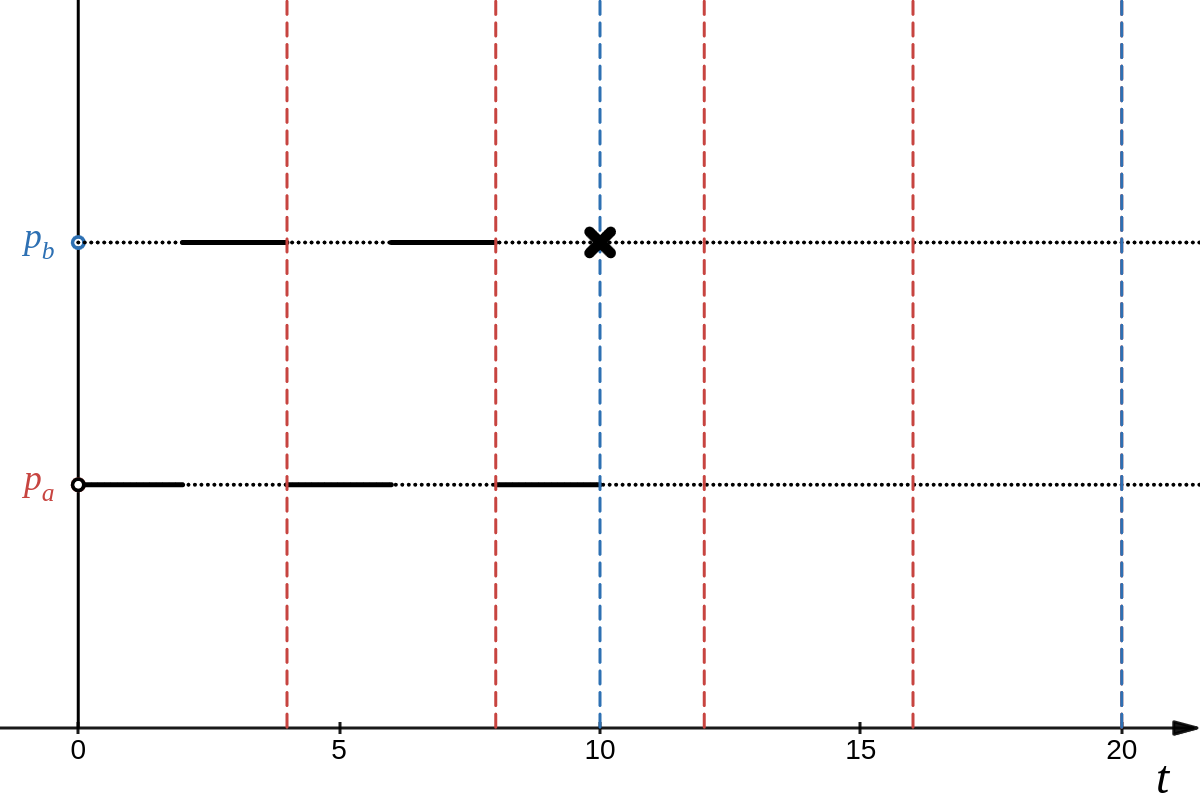
\includegraphics[scale=0.3]{../figures/rm_pre_fail.png}
\end{center}

A questo punto è $p_b$ ad andare in overflow! All'istante $t = 10$ infatti non siamo riusciti a completare le sue 5 unità temporali per completare l'esecuzione.

Abbiamo chiaramente incontrato un insieme di processi non schedulabili con priorità statica, e nemmeno introducendo la preemption abbiamo risolto il problema: dovremo trovare una qualche altra soluzione.

\subsubsection{Trattazione matematica}
Abbiamo che, nel caso dei due processi $p_a$ e $p_b$, il minimo che dobbiamo rispettare per poter in primo luogo eseguire i processi nel periodo di sistema è:
$$
n_a C_a + n_b C_b \leq T
$$
dove ricordiamo $T$ è il m.c.m. fra i periodi $t_a$ e $t_b$, e $n_a$ e $n_b$ sno rispettivamente il numero di volte in cui i processi $p_a$ e $p_b$ entrano in esecuzione per periodo di sistema.
In particolare, questi valori si possono calcolare dai perodi dei processi $\Delta t_a$, $\Delta t_b$, come:
$$
n_a = \frac{T}{\Delta t_a}, \quad n_b = \frac{T}{\Delta t_b}
$$

Sostituendo, si ha quindi:
$$
\frac{T}{\Delta t_a} C_a + \frac{T}{\Delta t_b} C_b \leq T \implies
\frac{C_a}{\Delta t_a} + \frac{C_b}{\Delta t_b} \leq 1
$$

Possiamo quindi generalizzare quanto trovato alla (ovvia) legge:
$$
U = \sum_{i = 0}^{n - 1} \frac{C_i}{T_i} \leq 1
$$
per $n$ processi arbitrari, dove $U$ viene detto \textbf{fattore di utilizzazione}.

Nell'esempio considerato finora, questo valore è:
$$
U = \frac{2}{4} + \frac{5}{10} = 1
$$
per cui i processi sono schedulabili. Ci manca da trovare un algoritmo che li sappia schedulare. 

\subsection{Algoritmo EDF}
L'algoritmo \textbf{EDF} (\textit{Earliest Deadline First}) è un algoritmo di schedulazione real-time, preemptive e a priorità dinamica.

Consiste nel mandare in esecuzione il processo che è più vicino alla sua deadline.
Come in tutti gli algoritmi a priorità dinamica, lo scheduler viene messo in esecuzione al cambio dei criteri di scelta (quindi quando un processo entra in coda pronti). In ogni caso, se due processi so trovano ugualmente vicini alla deadline al momento dell'esecuzione dello scheduler, si opta per ridurre i cambi di contesto al minimo e mantenere in esecuzione quello che sta già eseguendo.

\par\smallskip

Vediamo come questo algoritmo si applica all'esempio schedulabile visto finora:
\begin{center}
	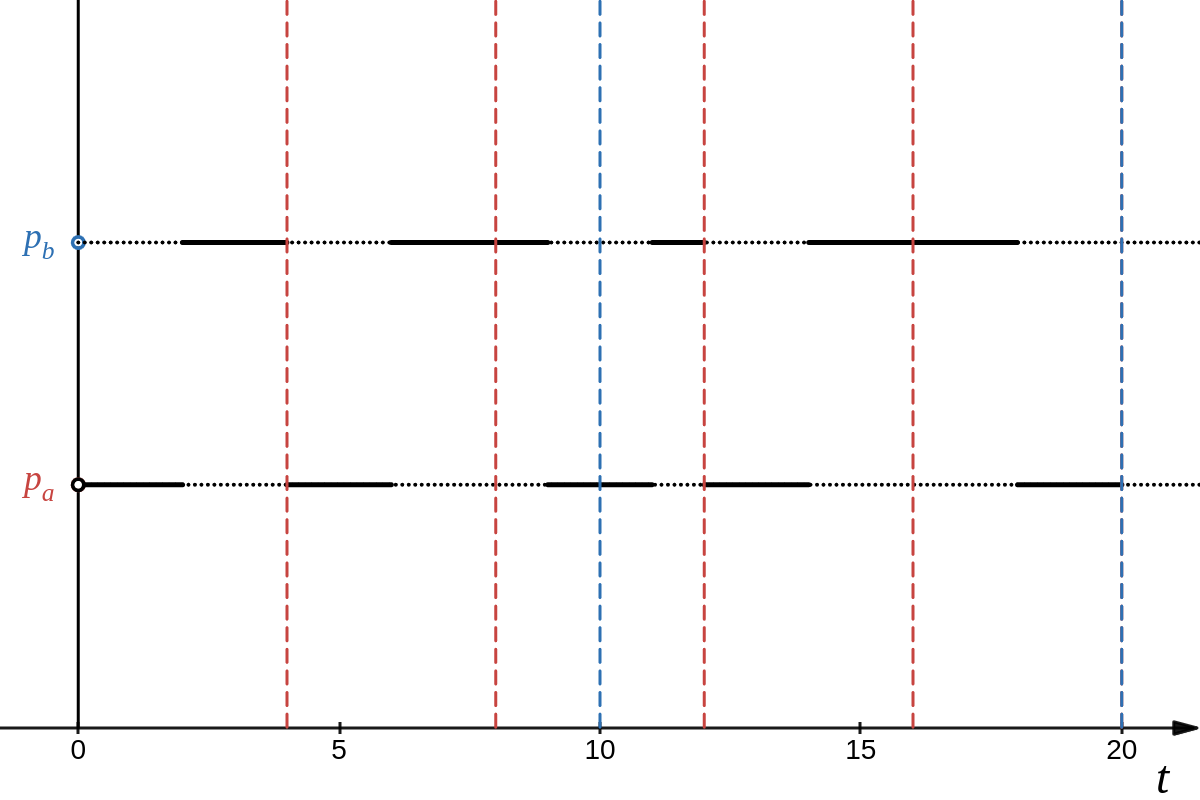
\includegraphics[scale=0.3]{../figures/edf.png}
\end{center}

Vediamo come otteniamo il 100\% dell'utilizzazione CPU, e riusciamo a schedulare i processi senza overflow.

All'istante $t = 8$, infatti, il processo $p_b$ è più vicino di $p_a$ alla deadline, e quindi viene mantenuto in esecuzione (fino a $t = 9$ dove termina).
In questo modo si riesce ad evitare che il suo CPU burst venga \textit{"tagliato"} prima che esso possa rispettare la sua deadline.

\par\smallskip

Abbiamo quindi trovato un'algoritmo che risolve i problemi che avevamo incontrato con RM: possiamo anticipare che questo algoritmo è ottimo fra gli algoritmi di schedulazione in real-time a priorità dinamica.

Una considerazione può essere fatta sull'overhead che introduciamo, almeno per l'esempio sopra. Abbiamo detto che sì, si cerca di mantenere al minimo i cambi di contesto, ma c'è comunque un certo overhead dato dall'esecuzione dello scheduler ad ogni creazione di processo.

In questo, potremmo aggiornare il modello introdotto in 9.1.1 come segue:
$$
U = ... \leq 1 - O_v 
$$
dove $O_v$ è un fattore temporale che tiene conto dell'overhead.

\subsection{Thread}
Introduciamo semplicemente il concetto di \textbf{thread} (o \textit{processo leggero}).
Avevamo detto che un processo è al contempo:
\begin{itemize}
	\item Un elemento che possiede delle \textit{risorse};
	\item Un elemento a cui viene \textit{assegnata} la CPU (si conserva lo \textit{stato} e si usa uno \textit{scheduler} per decidere quando caricarlo).
\end{itemize}

Possiamo separare questi due aspetti:
\begin{itemize}
	\item Definiamo \textbf{processo leggero}, o \textit{thread}, l'elemento a cui viene assegnata la CPU;
	\item Di contro, definiamo \textbf{processo pesante}, o \textit{task}, l'elemento che possiede le risorse.
\end{itemize}

Un processo pesante può essere composto da più thread, ognuno dei quali rappresenta effettivamente un flusso di esecuzione a sé stante. Tutti i thread possono però accedere alle risorse del loro processo pesante (incluso \textit{spazio di indirizzamento}, file aperti, ecc...). 

\end{document}
